\chapter{Lecture 9}

This lecture is about \texttt{Ensemble Methods
[Bagging, Boosting and Random Forest]} where chapter \texttt{ESL Chapter 8.7, 10.1
and 15} should be looked upon.

\begin{itemize}
  \item Bootstrapping (recap)
  \item Theory behind and use of
  \begin{itemize}
    \item Bagging
    \item Boosting
    \item Random forest
  \end{itemize}
  \item Out-of-bag estimates (OOB)
\end{itemize}

\section{Chapter 8.7}

This chapter is about bagging with examples of Trees and simulated Data.

\section{Chapter 10.1}

This chapter is about boosting methods and an outline of the chapter

\section{Chapter 15}

This chapter is about Random Forests. We get a definition of Random Forests and details of Random Forests. We are introduced to Out of Bag samples, variable importance, proximity Plots and Random Forests and overfitting. Furthermore we are looking at analysis of Random Forests, the Variance and De-Correlation Effect, Bias and Adaptive Nearest Neighbors.

\section{Bootstrapping Reviewed}

\section{Bagging}

Many models built on bootstrap replicates of data. The output from all models aggregated into one output. \\

Bagging is using the bootstrap to improve predictions, where bagging averages predictions over a collection of bootstrap samples. Average many noisy but approximately unbiased models and thereby reduce the variance.

The Bagging algorithm

\begin{itemize}
  \item Make B bootstrap samples of size $N$
  \item For $b = 1$ to $B$ repeat step (a)
        \begin{description}
           \item[a] Fit a model using the b'th sample and make the prediction $\hat{y}_b$
         \end{description}
  \item The bagging estimate is then given by the average of the ensemble of $B$ predictors
      \[
        \hat{y}_\text{bagging} = \frac{1}{B} \sum_{b = 1}^{B} \hat{y}_b
      \]
\end{itemize}

from lecture \cite[p.~6-8]{lecture9} and \cite[p.~282]{friedman2016elements}.

The Bagging bias, from lecture \cite[p.~14]{lecture9}. The bias of bagged trees is the same as that of the individual trees, as the trees are identically distributed

\begin{equation}
  \begin{split}
     E(\hat{y} -y) =& E \left[ \frac{1}{B} \sum_{b=1}^{B} (\hat{y}_b -y)\right] \\
       = & \frac{1}{B} \sum_{b=1}^{B} E(\hat{y}_b -y) \\
       & E(\hat{y}_b -y) \quad b=1, ..., B
  \end{split}
\end{equation}

From \cite[p.~285]{friedman2016elements}, This suggests that bagging—drawing samples
from the training data— will often decrease mean-squared error.

Then the bagging variance from lecture  \cite[p.~15]{lecture9}

The variance of the average of bagged estimates is ($\rho$ is the
correlation between pairs of trees)

\[
    \rho \sigma^2 + \frac{1- \rho}{B} \sigma^2
\]

The second term goes to zero as $B$ increases. We see that the size of the correlation between pairs of bagged trees, $\rho$, is what limits the variance reduction.

The Bagging method is Particularly good for high-variance, low-biased methods - such as trees.

\begin{itemize}
  \item Regression: The regression trees are fitted to bootstrap samples of the training data. The result is the average over all of the trees.
  \item Classification: A committee of trees each cast a vote for the class - and the majority vote is used as the prediction.
\end{itemize}

\section{Boosting}

\begin{itemize}
  \item Average many trees, each grown to reweighted versions of the training data.
  \item Weighting decorrelates the tree, by focusing on regions missed by past trees.
\end{itemize}

A set of weak classifiers (small trees) are grown in an adaptive
manner to remove bias (hence they are not independent).

Weights are put on the observations where the weights are updated to emphasize misclassifications.

The final estimator is a weighted average of all the trees.

Boosting shrinks bias. Therefore, combine small trees (stubs) with high bias. Many stubs together form a (very) good model with Boosting


The AdaBoost.M1 algorithm, the predictions from all of them are then combined through a weighted majority vote to produce the final prediction:

\[
    G(x) = sign \left( \sum_{m=1}^{M} \alpha_m G_m (x) \right)
\]

Here $\alpha_1, \alpha_2, ... , \alpha_M$ are computed by the boosting algorithm, and weight the contribution of each respective $G_m(x)$. Note that 


\[
    G_m(x) \in \{-1, 1\}
\]

\begin{figure}[H]
  \centering
  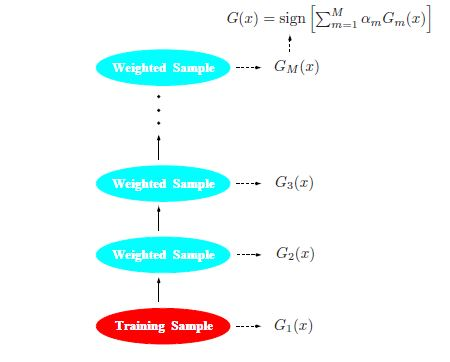
\includegraphics[width=0.9\textwidth]{adaboostalgorightm}
  \caption{Schematic of AdaBoost. Classifiers are trained on weighted versions of the dataset, and then combined to produce a final prediction}\label{fig:adaboostalgorightm}
\end{figure}

Basically the algorithm is

\begin{itemize}
  \item Initialize the observation weight $w_i = 1/N$, $i = 1, 2, ... , N$
  \item For $m=1$ to $M$:
  \begin{itemize}
    \item Fit a classifier $G_m(x)$ to the training data using the weights $w_i$
    \item Compute the weighted error of the newest tree
    \[
        err_m = \frac{\sum_{i=1}^{N} w_i \bm{I} (y_i \neq G_m(x_i))}{\sum_{i=1}^{N} w_i}
    \]
    \item Compute $\alpha_m = \log [(1 - err_m) / err_m ]$
    \item Update weights for $i = 1,...,N$
    \[
        w_i \leftarrow w_i \cdot \exp( \alpha_m \cdot \bm{I}(y_i \neq G_m(x)) )
    \]
    and renormalize to $w_i$ to sum to 1
  \end{itemize}
  \item Output $G(x) = sign \left[ \sum_{m=1}^{M} \alpha_m G_m(x) \right]$
\end{itemize}

From lecture \cite[p.~27]{lecture9} then boosting was intended as a committee method like Bagging.

Is a committee of weak learners where each cast a vote for the
final prediction. However, these evolve over time and the
members cast a weighted vote. 

Boosting dominates Bagging on most problems, and therefore
became the preferred choice.

\subsection{Shrinkage in Boosting}

Shrinkage, like ridge, can be added by controlling the learning rate, meaning the contribution of each tree is scaled by a factor $0 < \nu < 1$ 

\section{Random Forests}

Random forests is in lecture \cite[p.~33]{lecture9} and book \cite[p.~587]{friedman2016elements} 

It is 

\begin{itemize}
  \item Refinement of bagged trees
  \item Random forest tries to improve on bagging by decorrelating the tree, and reduce the variance
\end{itemize}

The algorithm for random forest algorithm

\begin{itemize}
  \item Define number of trees, B. Typically a few hundred (overfitting is not a problem)
  \item For $b=1$ to $B$ repeat the steps below
  \begin{itemize}
    \item Take a random sample of size N with replacement from the data (bootstrapping).
    \item Repeat until minimum node size, $n_{\text{min}}$ is reached (do not prune):
        \begin{itemize}
          \item Take a random sample without replacement of the predictors (of size $m < p$)
          \item Construct the first CART partition of the data (pick the best split among the $m$ variables)
        \end{itemize}
  \end{itemize}
  \item Output: B tress
\end{itemize}

If the variables are identically distributed, but not necessarily independent, with positive pairwise correlation $\rho$, the variance of the average is 

\[
    \rho \sigma^2 + \frac{1 - \rho}{B} \sigma^2
\] 

As B increases, the second term disappears, but the first remains, and hence the size of the correlation of pairs of bagged trees limits the benefits of averaging from  \cite[p.~588]{friedman2016elements} 

From lecture \cite[p.~37]{lecture9} then for, \textbf{classification} drop data down each tree in the forest and classify according to majority vote of B trees. For \textbf{regression} drop data down each tree in the forest and prediction is

\[
    \hat{y} = \frac{1}{B} \sum_{i=1}^{B} T_b (x)
\] 

where $T_b (x)$ is the estimate of $x$ for each b'th random tree.

\subsection{Out of bag samples}

With lecture \cite[p.~38]{lecture9} and \cite[p.~592]{friedman2016elements} then an important feature of random forests is its use of \textit{out-of-bag} (OOB) samples.

The OOB estimates

\begin{itemize}
  \item Samples not included in each bootstrap sample are called out-of-bag (OOB) samples.
  \item These can fairly be used for assessing individual tree performance!
  \item Using OOB samples for their corresponding trees, we obtain a missclassification rate.
  \item Results are similar to cross validation.
  \item OOB samples provide a way of constructing trees in a single sequence.
    \item As the forest is growing:
    \begin{itemize}
      \item Assess prediction error using OOB samples.
      \item Stop when error no longer decreases.
    \end{itemize}
\end{itemize}

\section{More on comparisons}

\begin{itemize}
  \item $n \ll p$
  \item Variable importance \cite[p.~593]{friedman2016elements}
  \item Proximity plots \cite[p.~595]{friedman2016elements}
\end{itemize}

So a note about \textbf{Bias and variance}. 

Bagging and Random Forests have the same bias as the bias of an
individual tree. This means that the gain obtained in prediction is due to variance reduction.

Boosting lowers bias as well as variance. Hence, we can use small
trees.

\subsection{Connection to ridge}

In ridge regression we see a similar bias-variance trade-off which indicates that bagging and random forests are suitable for $n \ll p$ problems. \cite[p.~38]{lecture9}

The ensamble averaging in RF reduces the contribution of any one variable much like the shrinkage in ridge regression and this is particular when $m$, the number of candidate variables in each split, is small.

But what when we have more variables than observations? e.g. $p > n$ \cite[p.~47-49]{lecture9}. 

Then two measures, The Gini index and OOB estimate. 

\begin{itemize}
  \item Gini: The improvement in the split-criterion at each split is accumulated over all the trees for each variable.
  \item OOB: Measures prediction strength by first dropping the OOB sample down the tree, then permuting the values for the $j$'th variable and computing the prediction accuracy again. An average of the difference in accuracy for all the trees gives the measure of importance for variable $j$.
\end{itemize}

Variable importance for a
random forest classification.
The left plot is based on the
Gini index whereas the right
plot is based on OOB
randomization.
The OOB approach tends to
spread the importance more
uniformly. The rankings are
usually similar.

\begin{figure}[H]
  \centering
  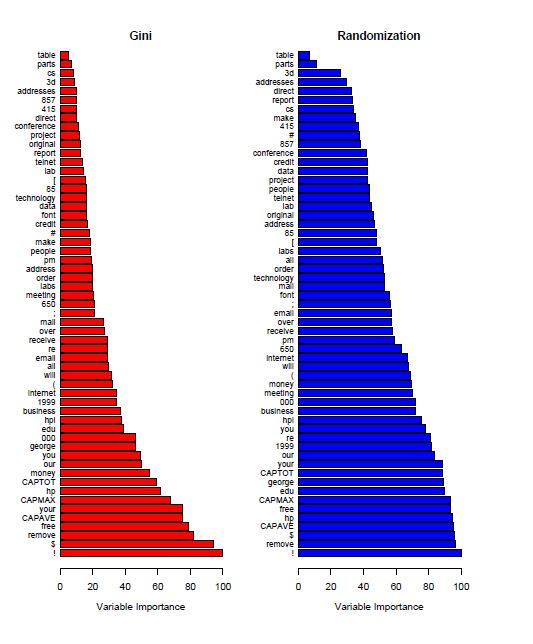
\includegraphics[width=0.9\textwidth]{ginivsoobRFplot}
  \caption{Variable importance plots for a classification random forest grown on the spam data. The left plot bases the importance on the Gini splitting index, as in gradient boosting. The right plot uses oobrandomization to compute variable importances, and tends to spread the importances more uniformly.}\label{fig:ginivsoobRFplot}
\end{figure}

\subsection{Proximity matrix and plots}

\begin{itemize}
  \item An $n \times $ proximity matrix is created by increasing the proximity value between two OOB samples by one when they end up in the same terminal node.
      \begin{itemize}
        \item Hence, a large value in (i; j) reflects that observation i and j are similar according to the classifiers.
      \end{itemize}
  \item The proximity matrix can be represented in two dimensions using multidimensional scaling. The idea behind this is to find a low-dimensional representation which preserves the pairwise distances.
  \item In general the proximity plots look like stars where points far from the decision boundary are the extremities, and the points close to the boundary are near the center.
\end{itemize}

\subsection{Random forests and Overfitting}

More on \cite[p.~596]{friedman2016elements}
 